\chapter{Architecture\ifdraft{ (Joe K./Dan) (100\%)}{}}
\label{chapter:architecture}

The \emph{architecture} of a computing system, akin to the
architecture of a purely physical artifact like a bridge or a
building, is its high-level structure. Just as when designing a
bridge, many choices must be made when designing a computing system;
these choices are driven by the system's requirements, both technical
and non-functional, as well as by external factors such as the
availability or affordability of computing hardware or network
bandwidth. In this chapter we describe the architectural issues
associated with E2E-VIV systems, present a model encompassing the
various possible architectural choices for such systems, and briefly
explore some architectural variants.

It is important to note that we are \emph{not} making a concrete
recommendation for a specific E2E-VIV system architecture. The
cryptographic foundations of E2E-VIV protocols have been developed to
a point where we have fairly high confidence in their ability to
detect errors in election outcome (whether unintentional or malicious)
and protect ballot privacy.  However, E2E-VIV protocols do not prevent
such errors, and an implemented E2E-VIV system should minimize the
chances of there being such errors. For this reason, there are many
open engineering issues associated with actually building, running,
and maintaining an E2E-VIV system that fulfills its requirements in
the face of both routine/expected failures and a wide range of
security threats. Because of these open engineering issues,
architectural experimentation---preferably, empirical testing of
various possible architectures to determine the most appropriate
one(s) to deploy in real-world election scenarios---is vital to
actually implementing a successful E2E-VIV system.

\section{Non-Functional Requirements Forcing Architectural Factors}

Several non-functional requirements of E2E-VIV systems force the
inclusion or consideration of specific architectural factors. We
consider each of these in turn.

\subsection{Certification}

Voting systems in most jurisdictions are subject to certification
requirements. The EAC and NIST have developed a set of Voluntary
Voting System Guidelines (VVSG) at the federal level, and the EAC
launched a Voting System Testing and Certification Program in 2007;
prior to 2007, voting systems were typically tested and certified by
the National Association of State Election Directors (NASED). The
EAC's guidelines are voluntary; however, many jurisdictions have
mandated adherence to them, so an E2E-VIV system that is to be widely
deployed must follow them as well as any other state and local
guidelines.

Certification processes generally require that a specific
implementation of a system be presented to a certification laboratory;
in the E2E-VIV context, this would likely consist of a complete set of
source files, plus binaries built to run on specific platforms and
with specific external dependencies, and any custom hardware to be
used in the system. Certification is typically an expensive process,
often costing many times more than developing the system in the first
place. Moreover, certification generally applies only to the system as
submitted; any changes to the system require a full or partial
recertification at additional expense.

This certification regime presents a sharp contrast to today's typical
software lifecycle. Most modern software systems, especially those
developed using agile techniques, are updated frequently to address
implementation issues and respond to changing customer needs. For
example, since its first release in September 2008 the Google Chrome
web browser has seen 42 major releases---an average of about one every
two months---and many minor patch releases in between. That sort of
release cycle is simply not an option for an E2E-VIV system, unless the
voting system certification regime changes dramatically.
Architectural decisions made during the system's development must
therefore be undertaken with great care, because major architectural
changes will be extremely expensive.

\subsection{Abstraction}

The software in an E2E-VIV system must be high assurance, and must, as
discussed above, undergo a certification process before it can be used
in actual elections. Thus, the software must be designed and
implemented with a level of abstraction that enables the generation of
convincing evidence for its correctness. This requires development
techniques that emphasize formal specification and verification, which
divide the software system into relatively small components with
well-defined, well-constrained interfaces. Each component can then be
verified individually with respect to its specification; moreover,
component behaviors with respect to external communication can be
formally characterized in ways that allow for verification of composed
subsystems.

\subsection{Deployment}

There is a wide spectrum of possible deployment scenarios for an
E2E-VIV system, each of which leads to certain decisions about its
architecture. At one extreme, the servers for an E2E-VIV system could
be hosted on a bespoke server cluster, built from the ground up
specifically for the system and housed in a facility under the
physical control of electoral authorities or their authorized
representatives. At another extreme, the servers could be hosted on a
commodity cloud computing infrastructure such as Amazon EC2 or
Microsoft Azure where electoral authorities have no physical control
over the servers. A third extreme would see the system implemented in
a purely peer-to-peer fashion, with the system's functionality
distributed among all participating computers and no
specifically-designated servers. The choice within this spectrum has
significant impact on both system availability and system security
requirements.

\subsection{Threats}
\label{sec:threats}

Mitigating the potential threats to E2E-VIV systems also leads to
various architectural choices. The following are some of the threat
vectors and mitigation strategies that need to be considered.

\paragraph {Single Point of Failure.} Any single point of failure,
such as a single server that contains essential data without which the
system can no longer function, is a tempting target for
attack. Therefore, the architecture should attempt to minimize or
eliminate such failure points.

\paragraph{Easy DDoS Targets.} The use of fixed IP addresses (or
address ranges) for E2E-VIV system components can open the system to
denial of service attacks, limit deployment flexibility, and make it
more difficult to recover from failures. The architecture should be
chosen such that IP addresses need not be hard-coded; preferably, they
should be changeable on-the-fly (i.e., during a live election
scenario) if necessary to protect or restore system integrity.

\paragraph{DDoS Mitigation.} Content distribution and network
protection services such as CloudFlare \cite{CloudFlare}, which route
traffic for their clients through their own high-bandwidth global
content distribution networks, can detect and protect against DDoS
attacks. They can also provide other benefits, such as higher
availability and improved response time. Such services could easily be
used to deliver static data to clients in an E2E-VIV system; however,
although they support technologies such as WebSockets for dynamic
data, they cannot necessarily protect systems that have complex
back-end architectures and client-server interactions. It is unclear
whether such services can successfully be used for all interactions in
E2E-VIV systems without compromising privacy or other requirements;
even if it is possible, doing so would certainly require specific
considerations in the design of the system architecture.

\paragraph{Non-Standard Foundations.} One way of countering threats is
to build the system using non-standard foundational techologies. For
example, instead of being built atop general-purpose operating systems
like Linux or NetBSD, E2E-VIV system components could be implemented as
\emph{unikernels}~\cite{Madhavapeddy13}, effectively single-purpose
application/operating system combinations that run directly atop
hypervisors such as Xen~\cite{Xen}. Unikernels, written using
technologies such as Mirage~\cite{OpenMirage} and HalVM~\cite{HalVM},
have considerably less code than general purpose operating systems;
each one performs a specific task, and they communicate amongst
themselves in the same manner as machines in a distributed
system. This implementation style can improve security in general, by
reducing the effort required to demonstrate the security of each
component and by minimizing potential attack surfaces once the
components are deployed. 

\paragraph{Secure Multi-Party Computation (MPC).} A common situation
in distributed computing systems is that a number of systems, each
having its own secret information, want to collaboratively compute a
result based on all their secret information without sharing the
secret information itself. Secure multi-party computation (MPC)
enables exactly this, letting the individual parties to a computation
keep their local secrets while computing global functions. MPC
functionality can be useful in distributing trust among multiple
individuals or organizations in a complex system, mitigating a number
of possible threats; we describe the distribution of trust in more
detail in the following section.


\subsection{Distributing Trust}
\label{sec:trust}

The distribution of trust in an E2E-VIV system is critical: if the
system is not trustworthy, the election results generated by it are
inherently suspect. The following are descriptions of the various
aspects of the system that must be trusted, and some possible ways to
establish that trust.

\paragraph{Trusting the Electoral Authority.} 

In general, the electoral authority is responsible for the integrity
of the election outcome, the privacy of the votes, and the
availability of the election system. Most E2E-VIV systems do not
require the public to trust the electoral authority or election
technology (including election servers run by election officials or
any others assigned to this task by the electoral authority) to detect
election integrity problems. The systems are designed to enable the
public to detect integrity issues without requiring trust in electoral
authorities or election technology, as long as the website is secure
with the ability to detect tampering. Additionally, these systems
typically use threshold cryptography so that vote privacy is not
compromised as long as a minimum number of election officials behave
as required by the protocol. The use of threshold cryptography also
influences the ability of individual election officials to affect a
denial of services.

In threshold cryptography, the cryptographic keys that allow for
results to be generated by the election system are divided into some
number of shares, a smaller threshold number of which are required to
actually generate results. For example, the keys might be divided into
10 shares, each of which is entrusted to a different official and at
least 7 of which are required to generate the tally. This also means
that fewer than 7 officials cannot compromise vote secrecy. This
allows the election to proceed in situations where some of the
election officials are unable (due to accident, illness, etc.) or
unwilling (due to denial of service efforts to stall the election
outcome from being tallied) to produce the keys, as well as providing
a check against vote secrecy violations by requiring at least 7 of the
10 officials to collaborate in generating the tally. The check against
denial of service can be strengthened even further with public
ceremonies surrounding key generation, share distribution, and tally
generation so that the specific electoral officials involved are
publicly known and can be held accountable for efforts to stall the
tally computation and its verification.

Another mechanism to increase trust in the electoral authority is
access restriction; if the election system allows physical access only
via computing systems at specific, publicly-known and well-secured
locations, and only during specified time frames, it is far more
difficult for a corrupt official (or group of officials) to manipulate
the election results without being detected.

Finally, the use of an append-only public bulletin board to record
encrypted ballot information in a tamper-evident fashion, combined
with publication of sufficient information about the election protocol
to allow members of the public to validate that their own ballots were
cast as intended and counted as cast, also acts as a significant check
against corruption by the electoral authority.

\paragraph{Trusting the Software.} The software in an E2E-VIV system
must be trusted to fulfill the system's requirements. Making all
development artifacts freely available as open source is an important
step toward such trust, as it allows for independent verification that
the source code has been designed and implemented
appropriately. However, the mere fact that it is open source is not
enough to make a piece of software trustworthy; there must be evidence
that the running software actually corresponds to the open source
code, has passed all required testing, and has not been corrupted
after installation.

Several mechanisms are available for increasing the trustworthiness of
deployed software. One is code signing; the system vendor can
digitally sign the final binary distribution of the software and make
the signature public, allowing any observer with sufficient access (in
practice, this would likely be the electoral authority) to validate
the signature against the actual deployed binaries. Self-certification
is a variant on code signing, where the software computes a signature
on itself at startup time and compares it against a known value; this
can detect accidental corruption (data storage errors, spurious bit
flips, etc.) but generally not malicious corruption, because an
attacker that successfully corrupts any part of the software could
also corrupt its self-certification mechanism. Similarly, a voter
relies on the client to check the signature whether using code signing
or self-certification, and a malicious client can modify the software
and pretend it passed the signature check.

Proof-carrying code~\cite{Necula02} allows software to be shipped with
accompanying formal correctness proofs that can be easily verified by
a theorem prover or certifying compiler at runtime. Such proofs can
help increase the trustworthiness of software and can easily be
included in small critical sections of an E2E-VIV system, but are
impractical for verifying the correctness of the entire system.

Another way of increasing trust in the software is to ensure that all
implemented protocols are open, with publicly available
specifications, and that multiple redundant implementations of the
protocols are used throughout the system. Ideally, the redundant
implementations should have different low-level designs and be
implemented using different programming languages. Thus, in order to
corrupt the system, it would not be sufficient to corrupt a single
protocol implementation; instead, all the implementations would need
to be corrupted in a consistent way that could not be detected by
observing differences in their behaviors.

\paragraph{Trusting the Servers.} In addition to trust in the
software, trust in the servers on which the software runs is
critical. Perhaps unintuitively, one approach is to assume that the
servers can't be trusted and design all the protocols and processes in
the system appropriately given that assumption. The property of
\emph{software independence}---an undetected change or error in the
software must not cause an undetectable change or error in an election
outcome---is an example of this approach. Even if the software is
fully trusted, an untrusted server can corrupt it in arbitrary ways;
software independence doesn't stop such corruption, but does guarantee
that if it affects the election results, it will be detected.  E2E-VIV
systems are designed to be software independent.

Even though distrusting the servers is useful in ensuring robust
protocol and system design, steps should still be taken to make the
servers more trustworthy.  One way to do this is to minimize the
number of components that must be trusted; an example would be using
servers that support unikernel architectures, as described in
\autoref{sec:threats}, to ensure that there is little to no other
potentially vulnerable software software, including OS libraries,
running alongside the E2E-VIV components.

Another way to increase trust in the servers is to deploy them in a
dynamic, possibly public, cloud infrastructure. In this way, the
particular server responsible for any given part of the system at any
given time is unknown. Assuming that the entire cloud infrastructure
is not compromised (for example, by a corrupt high-level insider),
this can significantly reduce the likelihood of a successful attack
against the servers.

Designing the system with a fully peer-to-peer architecture can help
to increase its trustworthiness, as there will no longer be single
points of failure; moreover, as shown in the seminal Byzantine
Generals result~\cite{Lamport82}, corrupted peers in a distributed
system can always be detected as long as more than 2/3 of the peers
remain uncorrupted. With appropriate use of cryptography, that
fraction can be improved significantly such that, in the most extreme
case, even a single uncorrupted peer can detect corruption of the
entire rest of the peer network.

A more radical way of increasing trust in the server infrastructure as
a whole is to pervasively use MPC, such that no single server ever
needs to be completely trusted. While some servers may be corrupted,
they will be detectable, and with a suitably redundant system design
the non-corrupted servers will still be able to carry out the
necessary computations for the election.

\paragraph{Trusting the Network.} The Internet is inherently insecure,
so measures must be taken to ensure the integirity of the system's
Internet-based communications. The first and most obvious of these is
that all communication among components in the system should use the
TLS protocol. The certificates used to establish TLS connections
should be \emph{pinned}, meaning that when a client wants to connect
to a server, the client already has information about the server's
security certificate (or information about a set of certificates, if
more than one is acceptable). If an unexpected certificate is provided
by the server, even if the hostname on the certificate matches the
hostname of the server, the connection fails.

Certificates used in E2E-VIV systems should have signature chains that
involve not only a certificate authority (like Comodo, Symantec, etc.)
but also the electoral authority or other appropriate government
entity; requiring the electoral authority to be involved in the
signature chain ensures that certificates cannot be issued for
malicious purposes by a rogue certificate authority and used to
compromise a running E2E-VIV system.

Finally, all communications of critical information (ballot
information, voter information, logs, audit data, etc.) in the
system---even over TLS-encrypted connections---should be carried out
using custom cryptographic protocols, so that even in the unlikely
event of a TLS compromise the data is protected.

\paragraph{Trusting the Voting Client.} One clear ``weak link'' in the
security of an E2E-VIV system is the voting client, which must by
definition---regardless of its implementation technology---involve
untrusted machines belonging to individual voters. There are two
potential issues: first, the voting client software itself might be
corrupted, either in transit to a voter's machine or after
installation; second, a voter's computing environment might be
corrupted in a way that compromises the voter's interactions with the
software.

There are various ways to ensure that the voting client software
remains uncorrupted. One technique for doing so with native
applications is application signing, where each application binary is
digitally signed before distribution and the signature is checked at
runtime. Trusted Computing techniques such as remote attestation can
provide even stronger guarantees, but rely on the presence of a
Trusted Platform Module (TPM) in the voter's computer.  However, the
fact that TPMs are not universally deployed (for example, Apple has
not shipped a computer, tablet, or phone with a TPM since 2006) means
that E2E-VIV systems cannot rely on Trusted Computing techniques.

Implementing the voting client as a web application can alleviate some
concern about the corruption of distributed native application
binaries, but makes it more difficult to ensure the voting client's
integrity and reason about its behavior. One problematic aspect of web
applications is that JavaScript can be interpreted differently not
only across platforms, but also across browsers on the same platform;
there are currently four different mainstream JavaScript engines---V8
for Google Chrome, Spidermonkey for Mozilla FireFox, Nitro for Apple
Safari, and Chakra for Microsoft Internet Explorer---plus a host of
others used by other browsers on various platforms. In addition, the
JavaScript language itself is not particularly amenable to the types
of analysis required for high assurance software. Progress has been
made toward enabling high assurance JavaScript, including techniques
such as Certified JavaScript~\cite{JSCert}, several JavaScript tools
from the Center for Advanced Software Analysis~\cite{CASATools}, and
Microsoft Research's Crypto Verification Kit~\cite{CVK}. However,
significant research is still needed in this area.

One potential approach for implementing a high assurance voting client
as a web application is to start with a high-level language that
supports the sorts of analysis necessary to provide the required
correctness and security guarantees.  Mozilla's asm.js~\cite{asm.js}
is a strict subset of JavaScript that can be used as a target for
compiling such higher-level languages. One nice side effect is that
this subset of JavaScript is easy to reason about, and generally
behaves identically across JavaScript runtime environments. With some
research and tool development, it should be possible to develop a high
assurance voting client, compile it to asm.js, and deploy it as a web
application.

With respect to the second issue, corruption of the voter's computing
environment, there is a wide range of possible threats. One, which we
do not know how to address as part of an E2E-VIV system
implementation, is surreptitious logging/monitoring software that
records the voter's actions and transmits them to a third
party. Detection and prevention of such monitoring can be improved
through standard secure computing practices such as malware scanning
and the use of reverse firewalls (preventing the computer from making
outgoing connections that are not approved by the user or by system
security policies). However, we can only recommend that voters take
such protective measures, and the voting client software cannot detect
whether they are actually in place. Additionally, it is possible that
a rare effort towards such monitoring is not detected by malware
scanning or the use of reverse firewalls.

Another threat is posed by malicious web browsers or OS libraries that
may deceive the voter into taking unintended actions. Such malicious
code might do any or all of the following: manipulate the appearance
of the voting client such that a voter believes she has voted for a
particular candidate or choice when she has actually voted for a
different one; block or corrupt communications between the voting
client and the rest of the E2E-VIV system, causing the voter to
unintentionally spoil ballots or otherwise interfering with vote
casting; and spoof the client-side verification screens to make a
voter mistakenly believe she is voting when she is actually not
interacting with the rest of E2E-VIV system at all. Many of these
threats can be partially or completely mitigated through judicious use
of cryptography and good user interface design---for example,
prominent use of confirmation codes transmitted out-of-band, such as
via postal mail, to authenticate communications between the voter and
the system in both directions---but there will always be the
possibility of malicious action on the part of untrusted client
systems. A good E2E-VIV system will enable a voter to detect any such
effort that changes election outcome. Additionally, an E2E-VIV system
with dispute resolution will enable a voter to prove that there is a
problem.

\paragraph{Trusting the Data.} As previously discussed, communications
can be protected using TLS and custom cryptographic protocols.
However, the communicated data needs to be committed to stable storage
at some point, in order to be verified, tallied, and audited. Standard
database technology is inappropriate for this purpose because of the
data integrity, confidentiality, and provenance requirements that must
be met in an E2E-VIV system. Data must be encrypted at rest to protect
against straightforward physical theft of storage devices, and should
remain encrypted during as much of the system's computation as
possible to protect against manipulation or disclosure by either
malicious software or individuals with administrative access to the
data store.

One way to prevent data manipulation, or at least make it nearly
infeasible, is to effectively make critical data in the system ``write
once'' by using a technique like hash chaining to ensure its
integrity; if a piece of data is changed after being written, the hash
chain for all subsequently-recorded data must also be modified in
order to ``hide'' the change. This makes data manipulation far more
difficult, though still technically possible if the system is
sufficiently compromised and its usage is not closely monitored
(recomputing the entire hash chain would generally require significant
computational resources). Replication of the data and the hash chain
in multiple locations that must be accessed independently further
prevents manipulation.

One way to prevent inappropriate disclosure of data while retaining
the advantages of well-known and well-understood database technology
is to use a tool like CryptDB~\cite{Popa11}, which allows for storage
of and secure computation with encrypted data in standard database
systems like MySQL and Postgres. Other possibilities include novel MPC
frameworks like ShareMonad~\cite{Launchbury14} and partial or full
homomorphic cryptographic schemes such as ElGamal and BGV that enable
computation of encrypted results over encrypted data.

The use of a public append-only bulletin board with vote encryptions
published in a tamper-evident and encouraging voters and observers to
frequently check the board provides a means of detecting data
manipulation, while the above safeguards make it additionally
difficult.

\paragraph{Trusting the Voter.} The voter, like the voting client, is
a ``weak link'' in the security of an E2E-VIV system. It is possible
for voters to compromise their own authentication credentials
intentionally or otherwise, allowing others to vote on their behalf;
to falsely challenge their own legitimately cast votes either
maliciously or because of mistaken memory; and to be misled into
either ``voting'' on a system other than the actual E2E-VIV system or
missing the time window for ballot casting.

In an unsupervised system, voters are responsible for their own
security. However, the vast majority of people lack the knowledge and
tools necessary to keep their computers secure. The electoral
authority can strongly encourage certain security measures, such as
use of antivirus/antimalware software on appropriate platforms, manual
checking of SSL certificates to ensure that they are signed by the
electoral authority, and installation of up-to-date OS, browser, and
E2E-VIV system software and security patches. However, there will
inevitably be voters who do not follow these recommendations, and it
is generally not possible---especially if it is web-based---for the
E2E-VIV system to evaluate a voter's compliance with them and act
accordingly.  Moreover, even voters using completely uncorrupted
computers can fall victim to social engineering attacks such as
official-looking physical mailers with false voting codes and false
voting server information.\footnote{Social engineering attacks have
  often been used in non-Internet election scenarios, primarily with
  the goal of suppressing votes; durng the 2014 midterm election
  cycle, there were numerous reports of mailings directing voters to
  incorrect voting places, giving incorrect election dates and
  absentee ballot submission deadlines, and containing incorrect
  information about voter registration.}  Judicious selection of the
distribution mechanisms for credentials and challenge mechanisms for
votes may help mitigate these issues, at least to the extent that they
can make it more difficult for non-malicious voters to compromise
their own security.

It is very difficult---or perhaps impossible---to defend an E2E-VIV
system against individual voters who are determined (or compelled) to
compromise the security of their own votes; ``shoulder surfing'' and
``rubber hose'' attacks\footnote{These are both actual terms of art in
  the field of computer security. A ``shoulder surfing'' adversary
  monitors all the actions of the voter throughout the voting process,
  while an adversary employing a ``rubber hose'' attack extracts
  information from the voter or forces the voter to take particular
  actions by means of threatened or actual physical harm.} remain
feasible in any unsupervised voting environment, regardless of the
credential distribution mechanism, voting mechanism, or other
protocols implemented by the system.

\paragraph{Trusting the Cryptography.} One area where many purportedly
secure systems fall short is their cryptography; even with good
intentions and sound designs, it is easy to make small but critical
mistakes in cryptographic algorithm and protocol implementations that
completely compromise system security.

It is clearly essential that proofs be carried out for all novel
cryptographic protocols used in an E2E-VIV system. These proofs may be
carried out on paper, or may be mechanized such that they are
checkable by computers. Moreover, all cryptographic protocol
implementations must be verified against their specifications; if the
specifications are mechanized, it is easier to carry out this
verification, and is even possible to \emph{synthesize} the
implementation directly from the specification in a
correctness-preserving fashion.

It is also essential that only well-studied secure cryptographic
algorithms and pseudorandom random number generators (PRNGs) be used
in E2E-VIV systems. The need for secure cryptographic algorithms is
obvious; the fact that bad sources of randomness can cause many
vulnerabilities in the otherwise-sound cryptographic systems built
atop them is less so. Exploits related directly to weak or absent
random numbers have taken place in various real world systems,
including fraudulent transactions in European EMV (Chip and PIN)
payment systems, large-scale theft from Android-based Bitcoin wallets,
and a complete compromise of the PlayStation 3 game console's digital
signature process.

E2E-VIV systems may use cryptographic algorithms and PRNGs approved by
government agencies, such as those specified by NIST in the Federal
Information Processing Standards (FIPS), but should be restricted to
those that have also been extensively studied by non-government
entities to counter the appearance that the government has a ``back
door'' allowing it to defeat the system's cryptography.\footnote{As
  reported by the New York Times in late 2013, the NSA actually did
  insert a back door into the NIST-approved Dual\_EC\_DRBG PRNG (it
  has since been removed from the approved PRNG list) and has actively
  worked to insert similar back doors into other cryptographic
  systems.}  Similarly, hardware entropy generators such as the RdRand
functionality found in current Intel processors can be used to provide
entropy in an E2E-VIV system, but must not be the sole sources of
entropy; since they are opaque subsystems whose functional details are
not available for inspection, they may contain hidden weaknesses or
back doors. The output of such generators can be combined with other
entropy as seed input to other open-source secure PRNGs, as is
standard practice in most operating systems' random number generation
subsystems.

\paragraph{Trusting the Toolchain.} Ken Thompson, in his 1984 Turing
Award lecture ``Reflections on Trusting Trust'' \cite{Thompson84},
demonstrated a fundamental problem with trust in computing systems: an
attack against the toolchain (compilers, assemblers, linkers) used to
build a system can silently, and effectively undetectably, insert a
``back door'' or other corruption into the system. If this attack is
carried out successfully, inspection of the source code for the
toolchain itself and the source code for the system will show nothing
unusual; the corrupted toolchain binary introduces the corruption when
building itself, or when building the rest of the system, and also
corrupts all the tools that can be used to analyze the system
(disassemblers, binary dump tools, etc.) such that the corruption
remains hidden. Thompson himself successfully carried out such an
attack within Bell Labs, and similar attacks have occurred ``in the
wild'' against systems such as the Delphi development environment for
Windows application; with stakes as high as controlling national
election results, it is not a stretch to believe that such attacks
would be attempted against E2E-VIV systems.

There are multiple ways to mitigate the possible impact of such an
attack. One is to ensure that the system uses a diverse set of
implementations of key components, all based on the same specification
but with different source code, built with different compilers, and
preferably running on different hardware and OS platforms; corruption
of a single component, or even a small number of them, could then be
detected by the uncorrupted components, and the effort required to
corrupt the system as a whole would be much higher. Another is to
counter the possibility of Thompson-style exploits by using multiple
toolchains in the technique proposed by David A. Wheeler in his
Ph.D. thesis, ``Fully Countering Trusting Trust through Diverse
Double-Compiling'' \cite{Wheeler09}.

\subsection{Scalability}

An E2E-VIV system, particularly at the national level, must be able to
handle a wide range of demand. It is human nature that many voters
will wait until the last day, or even the last hour, of a voting
period to cast their votes. Moreover, it is likely that attacks
against the system---and thus, system activity in general---will
increase in intensity as the end of a voting period approaches. Thus,
while the system may see very little sustained activity for much of an
election period, it must be able to scale to extreme levels of
activity at peak times. The architecture must take this into account,
so that the system can be dynamically deployed on more computing and
network resources as need arises. This might be done either by
utilizing public cloud resources that support elastic demand or by
using private resources that can be brought on- and offline as
required.

\subsection{Availability}

E2E-VIV systems must exhibit high availability;
\autoref{chapter:required_properties} stated an explicit requirement
for 99.9\% uptime during election periods and the ability to recover
from generalized (i.e., not caused by natural disaster or malicious
attack on the system) failures in under 10 minutes, and higher
availability---including in the face of malicious attack---would be
preferable. There are a number of techniques for ensuring high
availablity of systems, including the use of services like those
provided by Cloudflare to handle traffic spikes and distributed denial
of service attacks. The system architecture should be constructed in a
way that does not foreclose the use of such techniques.

\subsection{Usability}

Usability, including accessibility for disabled voters, is of
paramount importance in an E2E-VIV system. Especially for the
voter-facing parts of the system, the choice of implementation
technology may have a significant effect on usability. Essentially,
choices may need to be made between using Web technologies, which have
significant advantages in terms of reach (cross-platform, able to be
used on various sizes of device), and native applications, which tend
to exhibit richer interaction design and support more accessibility
features. The architecture might also allow for both types of
implementation, potentially at the cost of additional architectural
complexity.

\section{Architectural Feature Model}

As we have seen, there are many considerations to take into account
when making architectural decisions about an E2E-VIV system. Here, we
model the various architectural dimensions, and the (possibly wide)
range of choices within each, to give a sense of the potential
solution space for a workable E2E-VIV system architecture.

The Business Object Notation diagram in \autoref{figure:arch-choices}
shows the architectural choices that need to be made; for each
attribute of the architecture, a list of possible choices is
provided. There are seven dimensions, each of which can take on a set
of values. The values are chosen from 2-element sets for four of the
dimensions, from a 3-element for one, and from 4-element sets for the
remaining two. Since each dimension must have at least one selection
(the empty set is disallowed), this yields a total of
$(2^2-1)^4\times(2^3-1)\times(2^4-1)^2=127,\!575$ possible
architectural variants.

\begin{figure}
\begin{center}
\lstinputlisting[style=bon,frame=lines]{architecture_resources/architecture-dimensions.bon}
\end{center}
\caption{A specification of the possible variants for an E2E-VIV system.}
\label{figure:arch-choices}
\end{figure}

The architectural dimensions we have identified are the following:

\begin{itemize}
\item \textbf{Distribution of Authority} \ Authority in the
  system---that is, the ``official'' set of data stored in the system
  and control over access to and manipulation of that data---can be
  centralized or distributed. Centralized authority eliminates
  concerns about data consistency, as data can only be manipulated by
  one entity, but may cause issues related to system responsiveness,
  availability, and reliability. Distributed authority eliminates a
  single point of failure at the expense of needing to ensure data
  consistency and integrity. It is also possible to implement a hybrid
  authority model, where authority is concentrated in a small set of
  entities relative to the system as a whole; this is technically
  distributed authority because it is spread across entities, but
  behaves like centralized authority from the perspective of most of
  the entities in the system.

\item \textbf{Cryptographic Protocols} \ The set of cryptographic
  algorithms and protocols used to protect voter privacy and insure
  ballot integrity is a critical component in any E2E-VIV
  system. Security characterizations of individual cryptographic
  algorithms (e.g., block ciphers such as AES, standard public key
  cryptosystems such as RSA, threshold cryptosystems such as ElGamal)
  can be found in the large body of cryptography literature, and the
  selection of individual algorithms is generally a matter of picking
  an appropriate algorithm and security strength for a given
  task. However, since novel cryptographic protocols such as those
  required to implement E2E-VIV systems are not widely used or studied,
  evidence must be provided for the security of any such protocols
  used in a deployed system. Such evidence can be provided in two
  basic ways: through ``paper'' proofs that are carefully checked by
  multiple experts, or, if the protocols are mechanized in a formal
  specification language, through proofs that are automatically
  generated by cryptography protocol verifiers such as ProVerif
  \cite{ProVerif}. In general, it would be preferable for all
  cryptographic protocols in the system to be mechanized, as evidence
  could be generated repeatably and easily regenerated in the event of
  minor protocol changes; however, there may be cases where this is
  impractical. Thus, the cryptographic protocols of the system may
  have ``paper'' specifications, be mechanized in a formal system, or
  some combination thereof. Moreover, their implementations may be
  verified against the specifications in various ways, or may be
  directly synthesized from the specifications in a way that
  guarantees correctness.

\item \textbf{Evidence of Correctness} \ The development of a high
  assurance system such as an E2E-VIV system proceeds from a
  specification, at some level of formality, to an implementation that
  is intended to fulfill the specification. Assurance that the
  implementation actually does fulfill the specification can generally
  be obtained in two ways. First, the implementation can be developed
  in a way such that it is mechanically tied to the specification; for
  example, code generation techniques and refinement techniques can be
  used to mechanically generate correct implementations from
  specifications. Second, the implementation can be developed ``by
  hand'' with a set of included assertions that are meant to establish
  that the specification is being faithfully implemented; these
  assertions may then be checked by code analysis tools when building
  the system, or may be automatically compiled into testing code that
  validates the assertions when running the system. In practice, while
  it is clearly desirable for as much of the implementation as
  possible to be mechanically generated from the specification, most
  high assurance systems use some combination of these two techniques.

\item \textbf{Implementation Type} \ Regardless of the choices made
  along any of the other dimensions, a reference for what constitutes
  a ``correct'' implementation must be provided. Either a ``golden
  im\-ple\-men\-ta\-tion'' with strong correctness guarantees or a
  complete set of open protocols and specifications may serve as such
  a reference.

  A golden implementation $G$ may be synthesized directly from a
  formal specification using semantics-preserving transformations, may
  be implemented in one of several languages using a ``correct by
  construction'' approach, or may be painstakingly verified against a
  formal specification either by hand or in an automated fashion. In
  any case, such a $G$ defines the correct behavior of the system but
  may---because of its implementation technology or other
  factors---not satisfy real-world performance requirements, memory
  usage/storage requirements, etc.  However, $G$ can be used as a
  reference point for other implementations; if the behavior of an
  implementation $X$, which does satisfy deployment requirements but
  for which we have no strong correctness guarantees, conforms to that
  of $G$, then $X$ is also a correct implementation (and is likely
  better suited for deployment).

  In the absence of a golden implementation, evidence for
  implementation correctness can come in the form of conformance
  testing against open protocols and specifications. This requires
  that such protocols and specifications are provided for the entire
  system in formats such that conformance checking is feasible.

\item \textbf{Key Distribution Method} \ In all the possible
  implementations of an E2E-VIV system, encryption keys will be
  required to fulfill security, privacy, and integrity
  requirements. The ways in which these keys will be generated is
  determined by the cryptographic algorithms chosen for use in the
  system, but the ways in which they are distributed depend on
  architectural choices. For example, public ``key generation and
  distribution'' ceremonies and the use of threshold cryptography for
  the keys that enable generation of the final tally, described in
  \autoref{sec:trust}, may be used to improve trust in the system and
  making it more resilient in the face of attempts by the electoral
  authority to determine votes or prevent the completion of the
  election tally or its audit. However, the generation and use of
  encryption keys in the system is not limited to the election
  authority; as a result of the pervasive use of TLS encryption for
  communication, keys are continually generated and exchanged
  throughout the system.

  The most widespread method of key distribution today is the public
  key infrastructure (PKI), which manages digital certificates and
  related artifacts. Trusted certificate authorities issue
  certificates that bind public keys with user or organizational
  identities; this is what allows a user to connect to her bank
  online, examine the certificate presented during the connection, and
  see that the certificate was in fact issued to her bank rather than
  a man-in-the-middle attacker. As described in \autoref{sec:trust},
  PKI can be used to guarantee to voters (in the event that they
  check) that their connections to an E2E-VIV system are secured using
  a certificate issued to and signed by the electoral authority. PKI
  is effectively mandatory for secure Internet connections using the
  TLS protocol, but may also be used to manage other keys in the
  system; however, this requires a trusted certificate authority for
  such keys. 

  Another method of key distribution is the ``web of trust'', first
  described by the creator of Pretty Good Privacy
  (PGP)~\cite{Zimmermann95} in 1992. Unlike a typical PKI system, a
  web of trust system does not have the concept of trusted certificate
  authorities; instead, it is essentially a large collection of public
  keys that can be digitally signed as a signal of trust. Each public
  key in the repository identifies an entity (individual or
  organization) that possesses the corresponding private key. Each
  public key can be digitally signed by the owners of other keys. For
  example, assume Alice and Bob have both published their public keys,
  which are $A$ and $B$ respectively. If Alice knows Bob personally,
  and Bob can demonstrate to Alice that his public key is actually
  $B$, then Alice can sign key $B$ (with her private key) to indicate
  her trust that key $B$ belongs to Bob. Such signatures build a
  distributed set of trust relationships: if Alice trusts Bob, and Bob
  trusts Charlie, then it is presumed that Alice can trust
  Charlie. This is similar to the way certificate authorities work in
  PKI systems; in effect, Bob acts as a certificate authority for
  Alice because of the trust relationship they have established, and
  Alice can trust any key that he has signed (or that has been signed
  by a key he has signed, etc.). Key distribution via a web of trust
  could be useful in various parts of E2E-VIV systems, as a means of
  collectively building trust relationships within the system rather
  than relying on the single points of failure inherent in PKI
  infrastructures.

\item \textbf{Deployment Style} \ The E2E-VIV software can be deployed
  in one of three ways: (1) servers run entirely on trusted servers
  managed by the electoral authority or its designated
  representatives, and client applications access the servers through
  well-defined, well-controlled interfaces; (2) servers run, in whole
  or in part, on public cloud infrastructure, while client applications
  still access them through well-defined interfaces; (3) the system is
  structured in a peer-to-peer fashion, where ``server'' functionality
  is distributed across all entities in the system and at least some
  of them run in an uncontrolled environment (i.e., voters'
  computers). 

\item \textbf{Client Technology} \ Implementation of the client
  software used by voters, as well as the administration software used
  by the electoral authority, can be done in two basic ways: (1)
  develop custom applications for the various hardware/OS platforms
  that will be used by voters and the electoral authority; or (2) use
  Web application technologies to develop a single Web-based
  application that will be accessible from all (reasonable)
  platforms. It is also possible to choose both implementation
  strategies for all applications (i.e., both voters and the electoral
  authority can access the system through either native applications
  or a Web application, as they choose) or make different choices for
  different applications (e.g., the voter application is implemented
  as a Web application while the electoral authority's administration
  application is implemented as a native application).

\end{itemize}

\section{Primary Architectural Variants}
\label{section:primary_architectural_variants}

Given the many dimensions of the architectural feature model, and
number of choices in each, the number of possible architectural
variants for the system is large. Here, we briefly discuss a few of
the primary system variants that can be described by the feature
model. Since we are only describing them at a high level, some of the
variants correspond to many possible feature selections in the feature
model (for example, they might have any of the different types of
correctness evidence or any of the different key distribution
methods).

\subsection{Mirrored Servers}

One possible architecture, which features centralized authority as its
primary defining characteristic, is the ``mirrored servers''
architecture depicted in \autoref{figure:arch-mirrored-servers}. The
double arrows in this diagram (and later diagrams in this chapter)
denote \emph{client} relationships (one entity making use of another's
services), while the thick double-ended arrows denote \emph{mirroring}
relationships (entities, or groups of entities, ensuring that their
states accurately reflect each other for redundancy or availability).

\begin{figure}[t]
\begin{center}
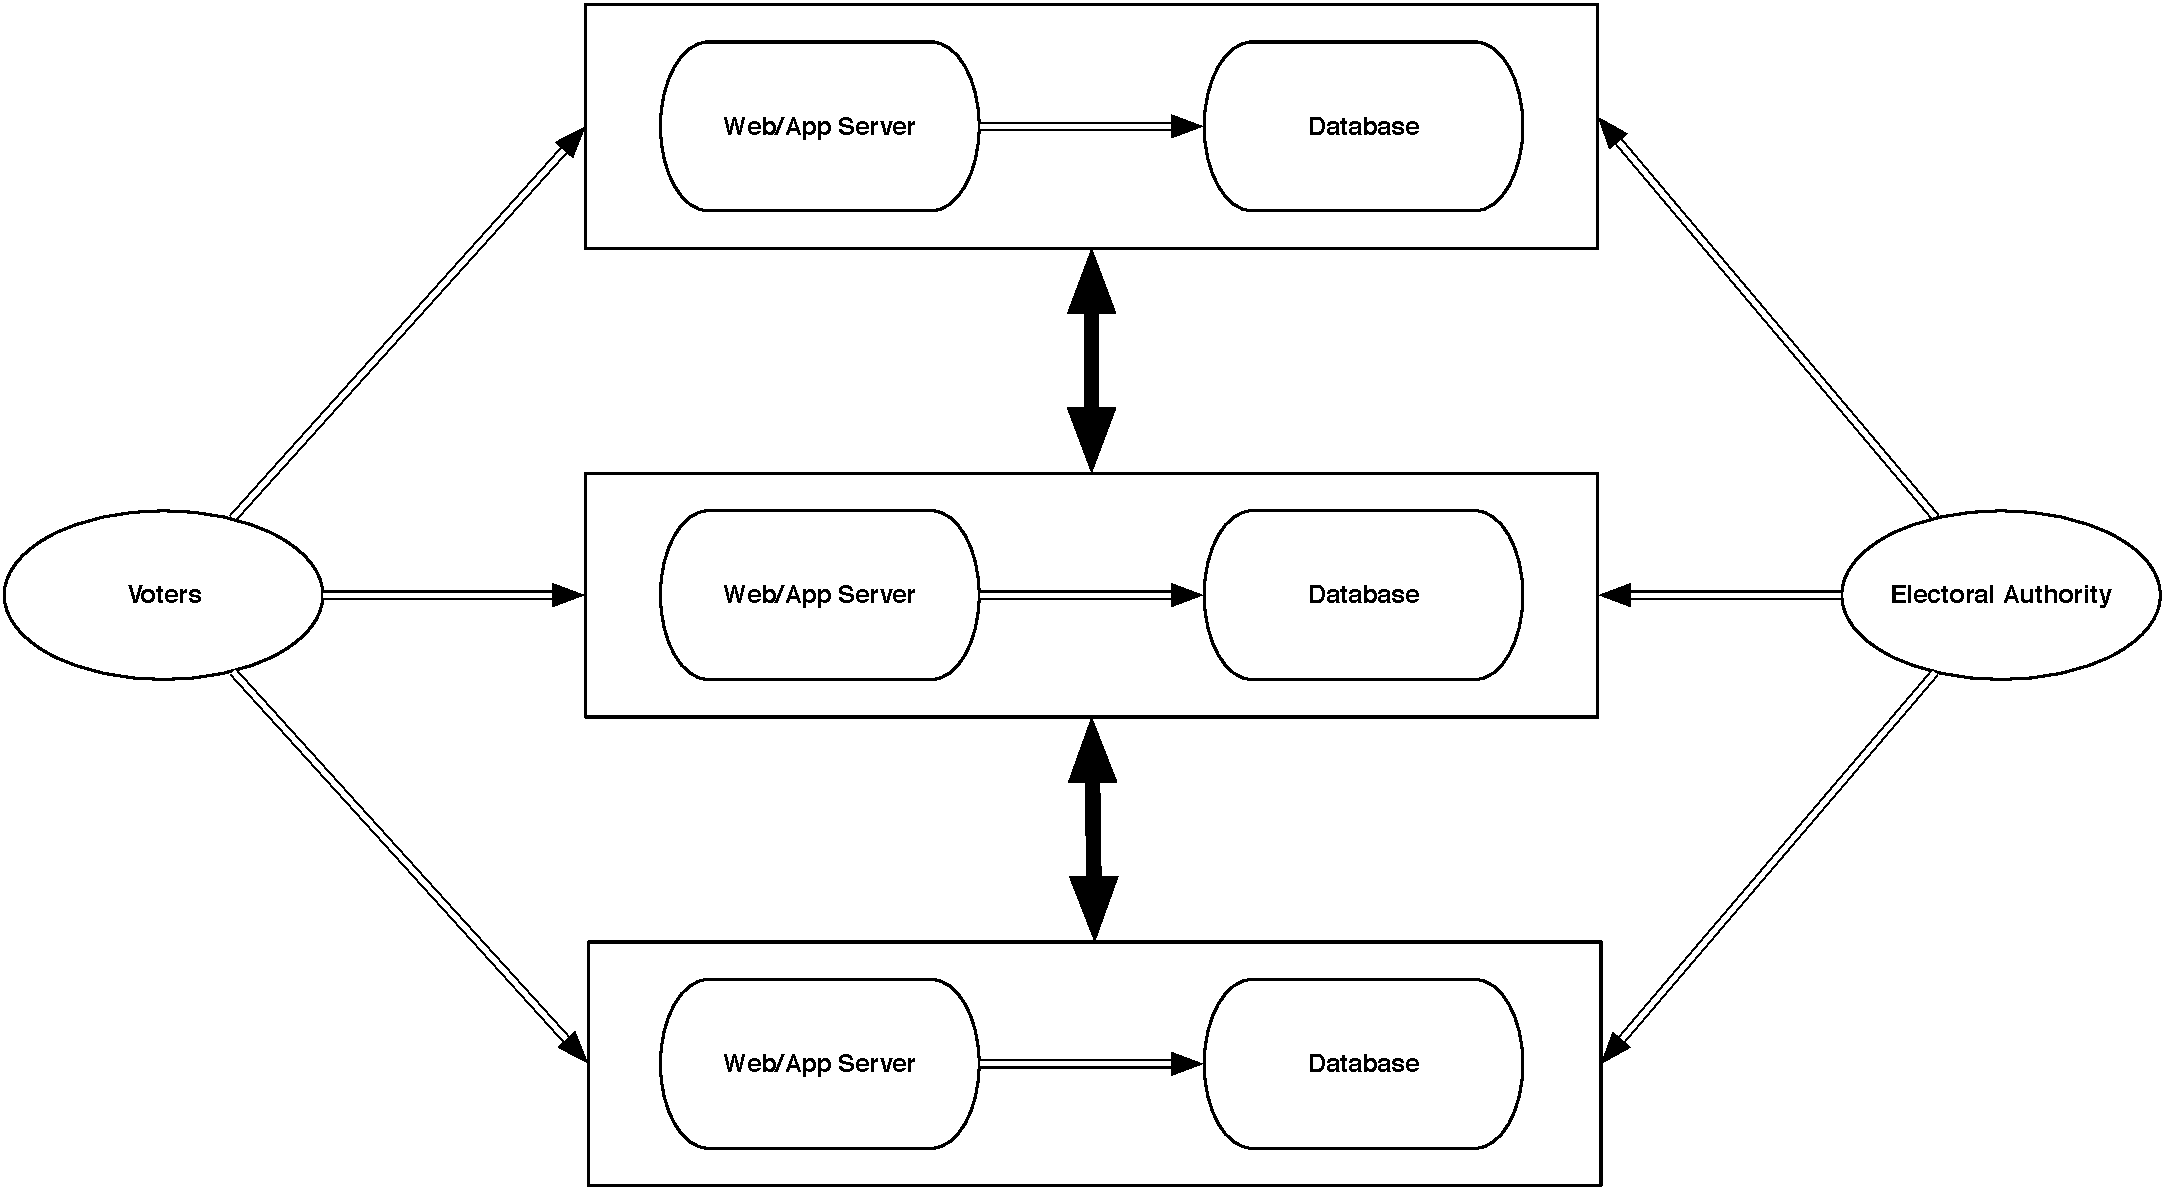
\includegraphics[width=6.5in]{architecture_resources/mirrored-servers.pdf}
\end{center}
\caption{An architecture with centralized authority and mirrored
  servers.}
\label{figure:arch-mirrored-servers}
\end{figure}

In this architecture the Web/App Server (to which voters, using either
a web-based interface or custom applications, connect to cast their
ballots) is a client of the Database, which stores all information
relevant to the operation of the E2E-VIV system (ballot styles, cast
and spoiled ballots, etc.). In an actual implementation, the
monolithic Database would likely be split into multiple databases
since the access patterns and performance needs for data such as
ballot styles, cast and spoiled ballots, voter lists, etc., are likely
to be quite different. There might also be more components within each
mirror (for example, separate servers for dealing with native
applications vs. web access in a system that supports both).

Regardless of the number of servers within each mirror, the mirroring
in this architecture is done primarily for availability and
reliability; it ensures that, as long as at least one set of mirrored
servers is running, the system can remain operational (albeit perhaps
at a degraded level of responsiveness). Authority is centralized in
the sense that each mirror has a complete set of data for the system
and behaves accordingly; one mirror is designated as the
\emph{primary} mirror and is considered the authoritative source of
information in the event of inconsistency. Voters and the electoral
authority access the system by interacting with an individual
(typically, the primary) mirror, and the entire set of mirrors appears
logically as a single server-side system.

\subsection{Large Fixed Set of Servers}

Another possible architecture, which introduces the potential for
distributed authority but still has the logical presentation of a
single server-side system, is a large fixed set of servers. This
architecture, an example of which is depicted in
\autoref{figure:arch-large-fixed-set-of-servers}, still features
mirroring for redundancy and availability; however, it allows for
flexible allocation of resources. For example, there might be twice as
many Web/App Server instances as there are Database instances, or
there might be more Database instances dealing with dynamic cast and
spoiled ballot data than dealing with fixed election definition data
such as ballot styles.

\begin{figure}[p]
\begin{center}
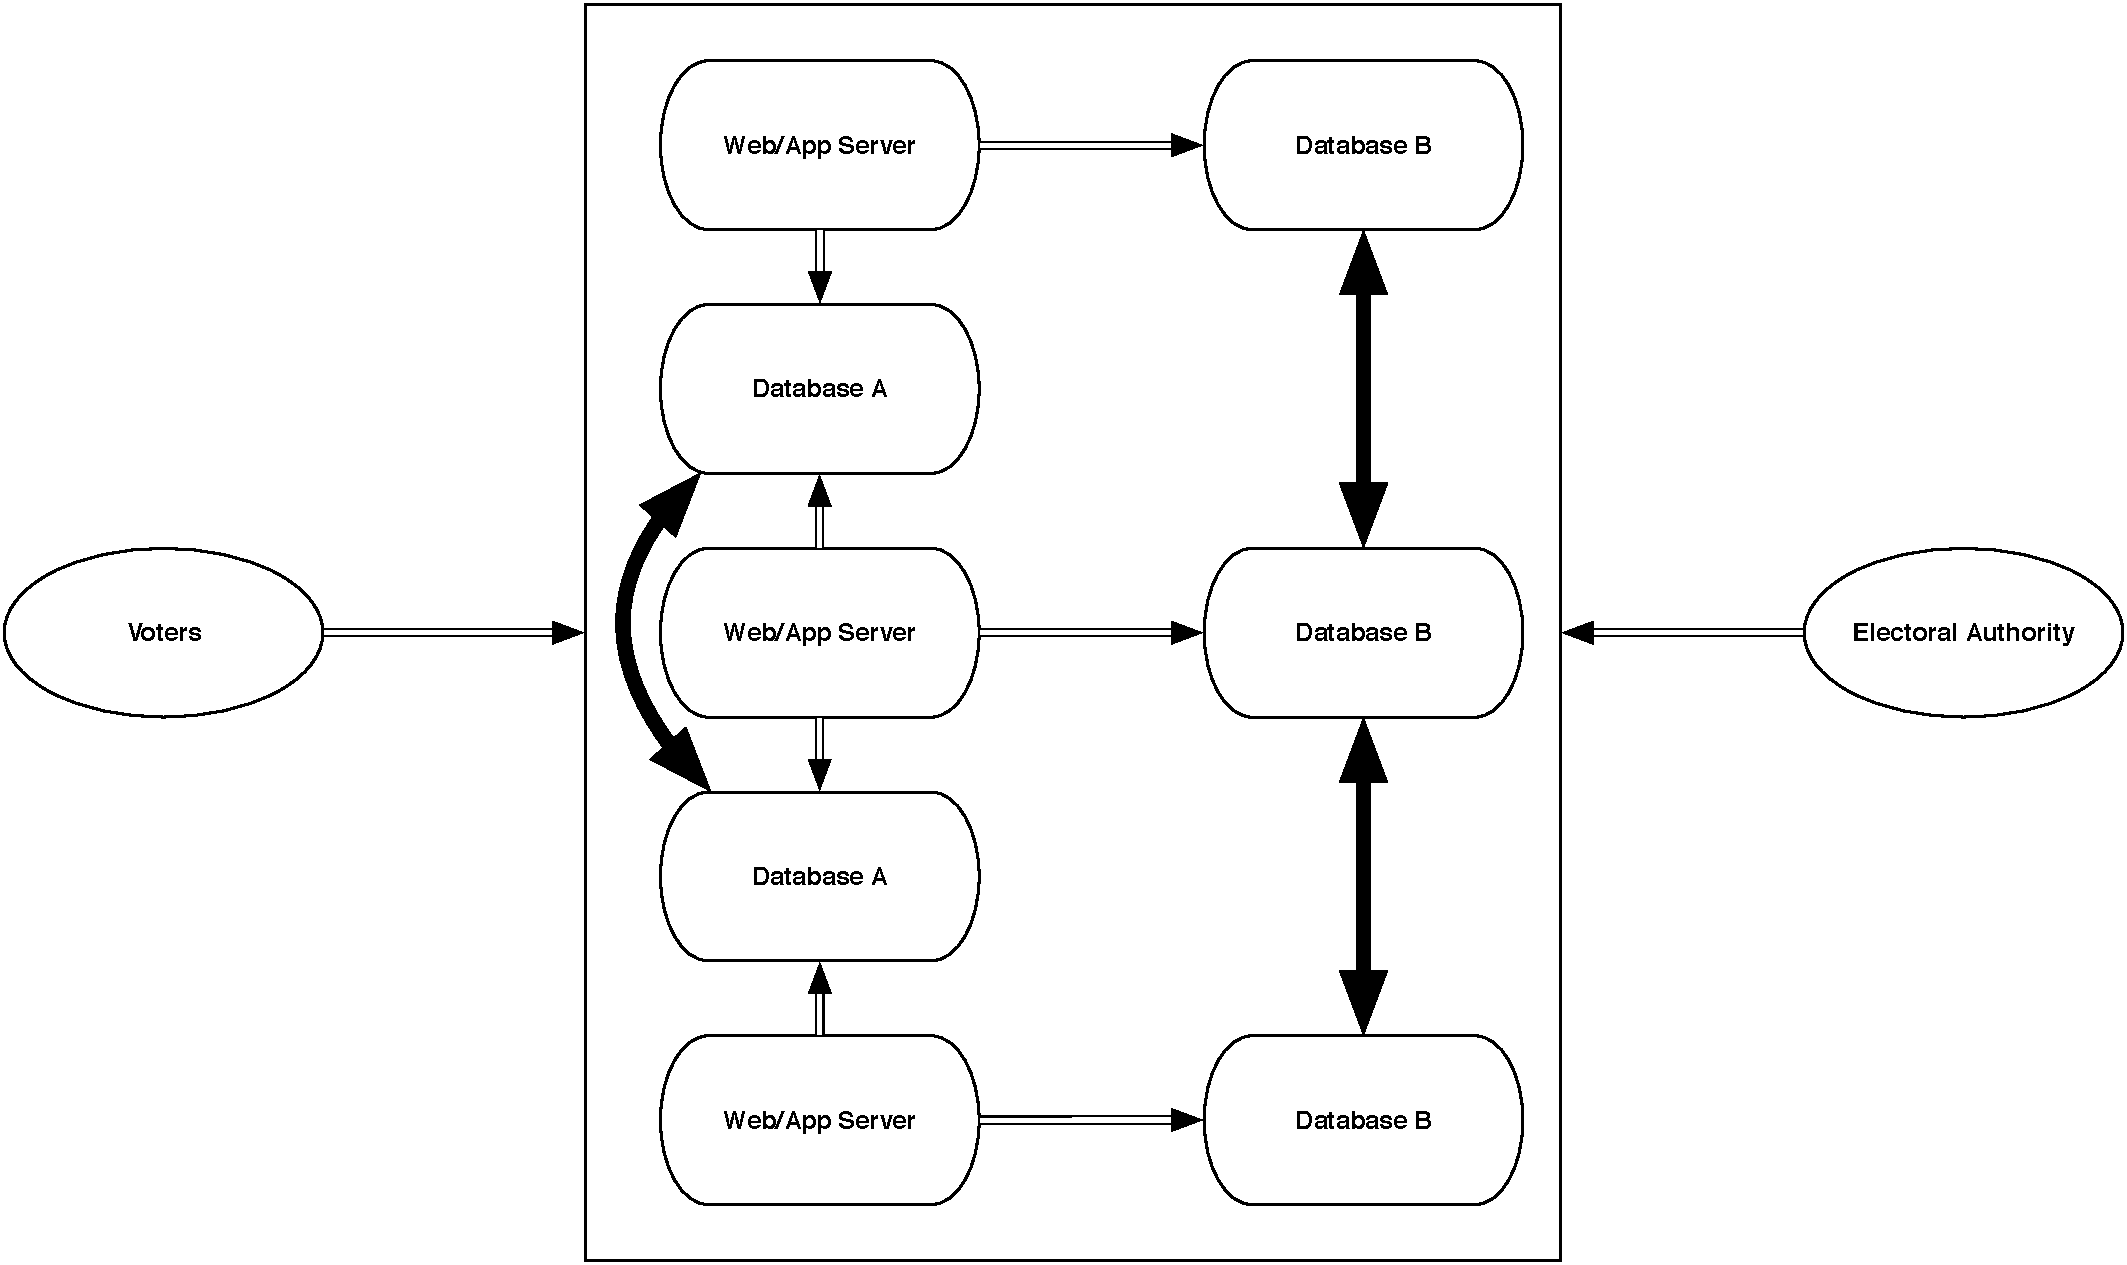
\includegraphics[width=6.5in]{architecture_resources/large-fixed-set-of-servers.pdf}
\end{center}
\caption{An architecture with a large fixed set of servers.}
\label{figure:arch-large-fixed-set-of-servers}
\end{figure}

\begin{figure}
\begin{center}
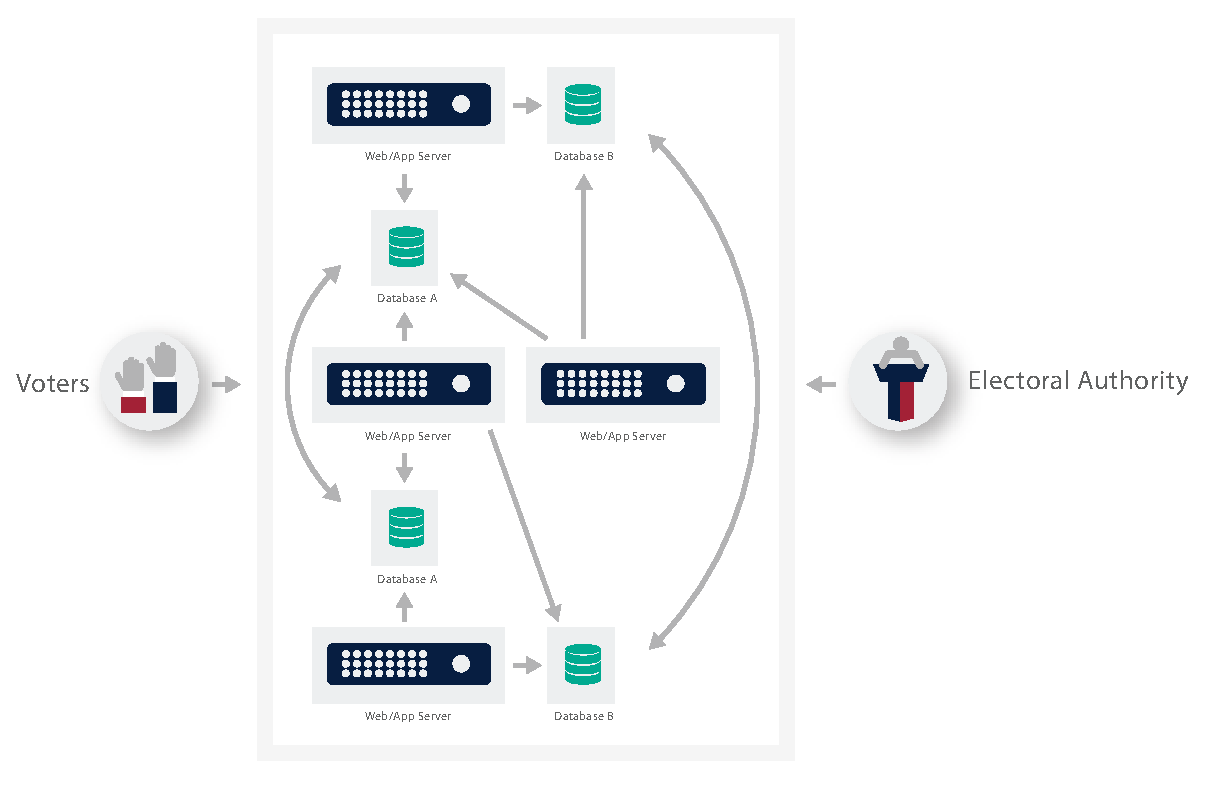
\includegraphics[width=6.5in]{architecture_resources/large-fixed-set-modified.pdf}
\end{center}
\caption{The same fixed set of servers as in
  \autoref{figure:arch-large-fixed-set-of-servers} performing a different
  allocation of tasks.}
\label{figure:arch-large-fixed-set-modified}
\end{figure}

The servers within this architecture could, amongst themselves, behave
as a peer-to-peer system, a set of client-server systems, or a set of
mirrors of various sizes for the purposes of providing high
availability and redundant storage and ensuring data consistency. A
key aspect of this architecture is that the number of servers, while
large, is fixed; this allows the topology of the servers and the
communications amongst them to be known at all times, making it
straightforward to monitor the system's health and performance and to
quickly detect any issues that arise.

As an example, \autoref{figure:arch-large-fixed-set-of-servers}---only
one of many possible server topologies in such an architecture---has
two separate mirrored Databases (one with two mirrors, and one with
three) being accessed by three separate Web/App Servers. If it is
determined that the Databases are underloaded and the Web/App Servers
are overloaded, one of the servers running Database B could easily be
repurposed to run an additional Web/App Server
(\autoref{figure:arch-large-fixed-set-modified}) without changing the
actual set of servers in the architecture and without compromising the
redundancy of data storage in the system.

While one possible deployment of this architecture would see every
server containing the full authoritative data set, it is far more
likely that each would contain only part of it and that the authority
in the system would, therefore, follow either a hybrid or a distributed
model. 

\subsection{Dynamic Cloud}

The two previous architectural variants involved the deployment of a
fixed set of servers, either as a collection of mirrors or in other
topologies. The next variant departs from these by deploying services
not across a fixed set of servers, but instead within a dynamic cloud
infrastructure, while still presenting itself as a single server-side
system for external interactions. Such an infrastructure allows for
the addition and removal of computing resources as necessary during
the operation of the system, using various distributed communication
and consistency protocols to deal with resource changes in a way that
is effectively invisible to the system's users while maintaining data
integrity and service
availability. \Autoref{figure:arch-dynamic-cloud-small,
  figure:arch-dynamic-cloud-large} show snapshots of a dynamic cloud
deployment at times when it has five and eleven running servers,
respectively. Note, in particular, that the client relationships among
the servers in the cloud may evolve over time as well; for example, in
\autoref{figure:arch-dynamic-cloud-small}, the server at the ``top''
of the cloud could establish direct communication with the server at
the ``bottom left'' of the cloud if necessary.

\begin{figure}[p]
\begin{center}
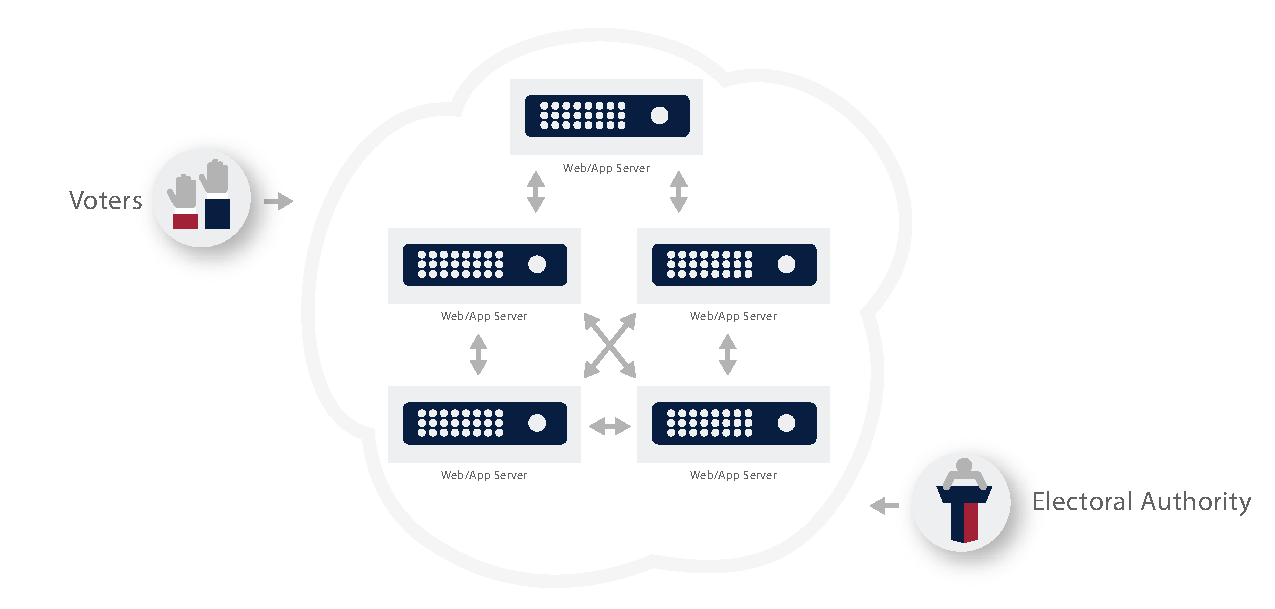
\includegraphics[width=5.5in]{architecture_resources/dynamic-cloud-small.pdf}
\end{center}
\caption{A dynamic cloud architecture with a small number of servers.}
\label{figure:arch-dynamic-cloud-small}
\end{figure}

\begin{figure}
\begin{center}
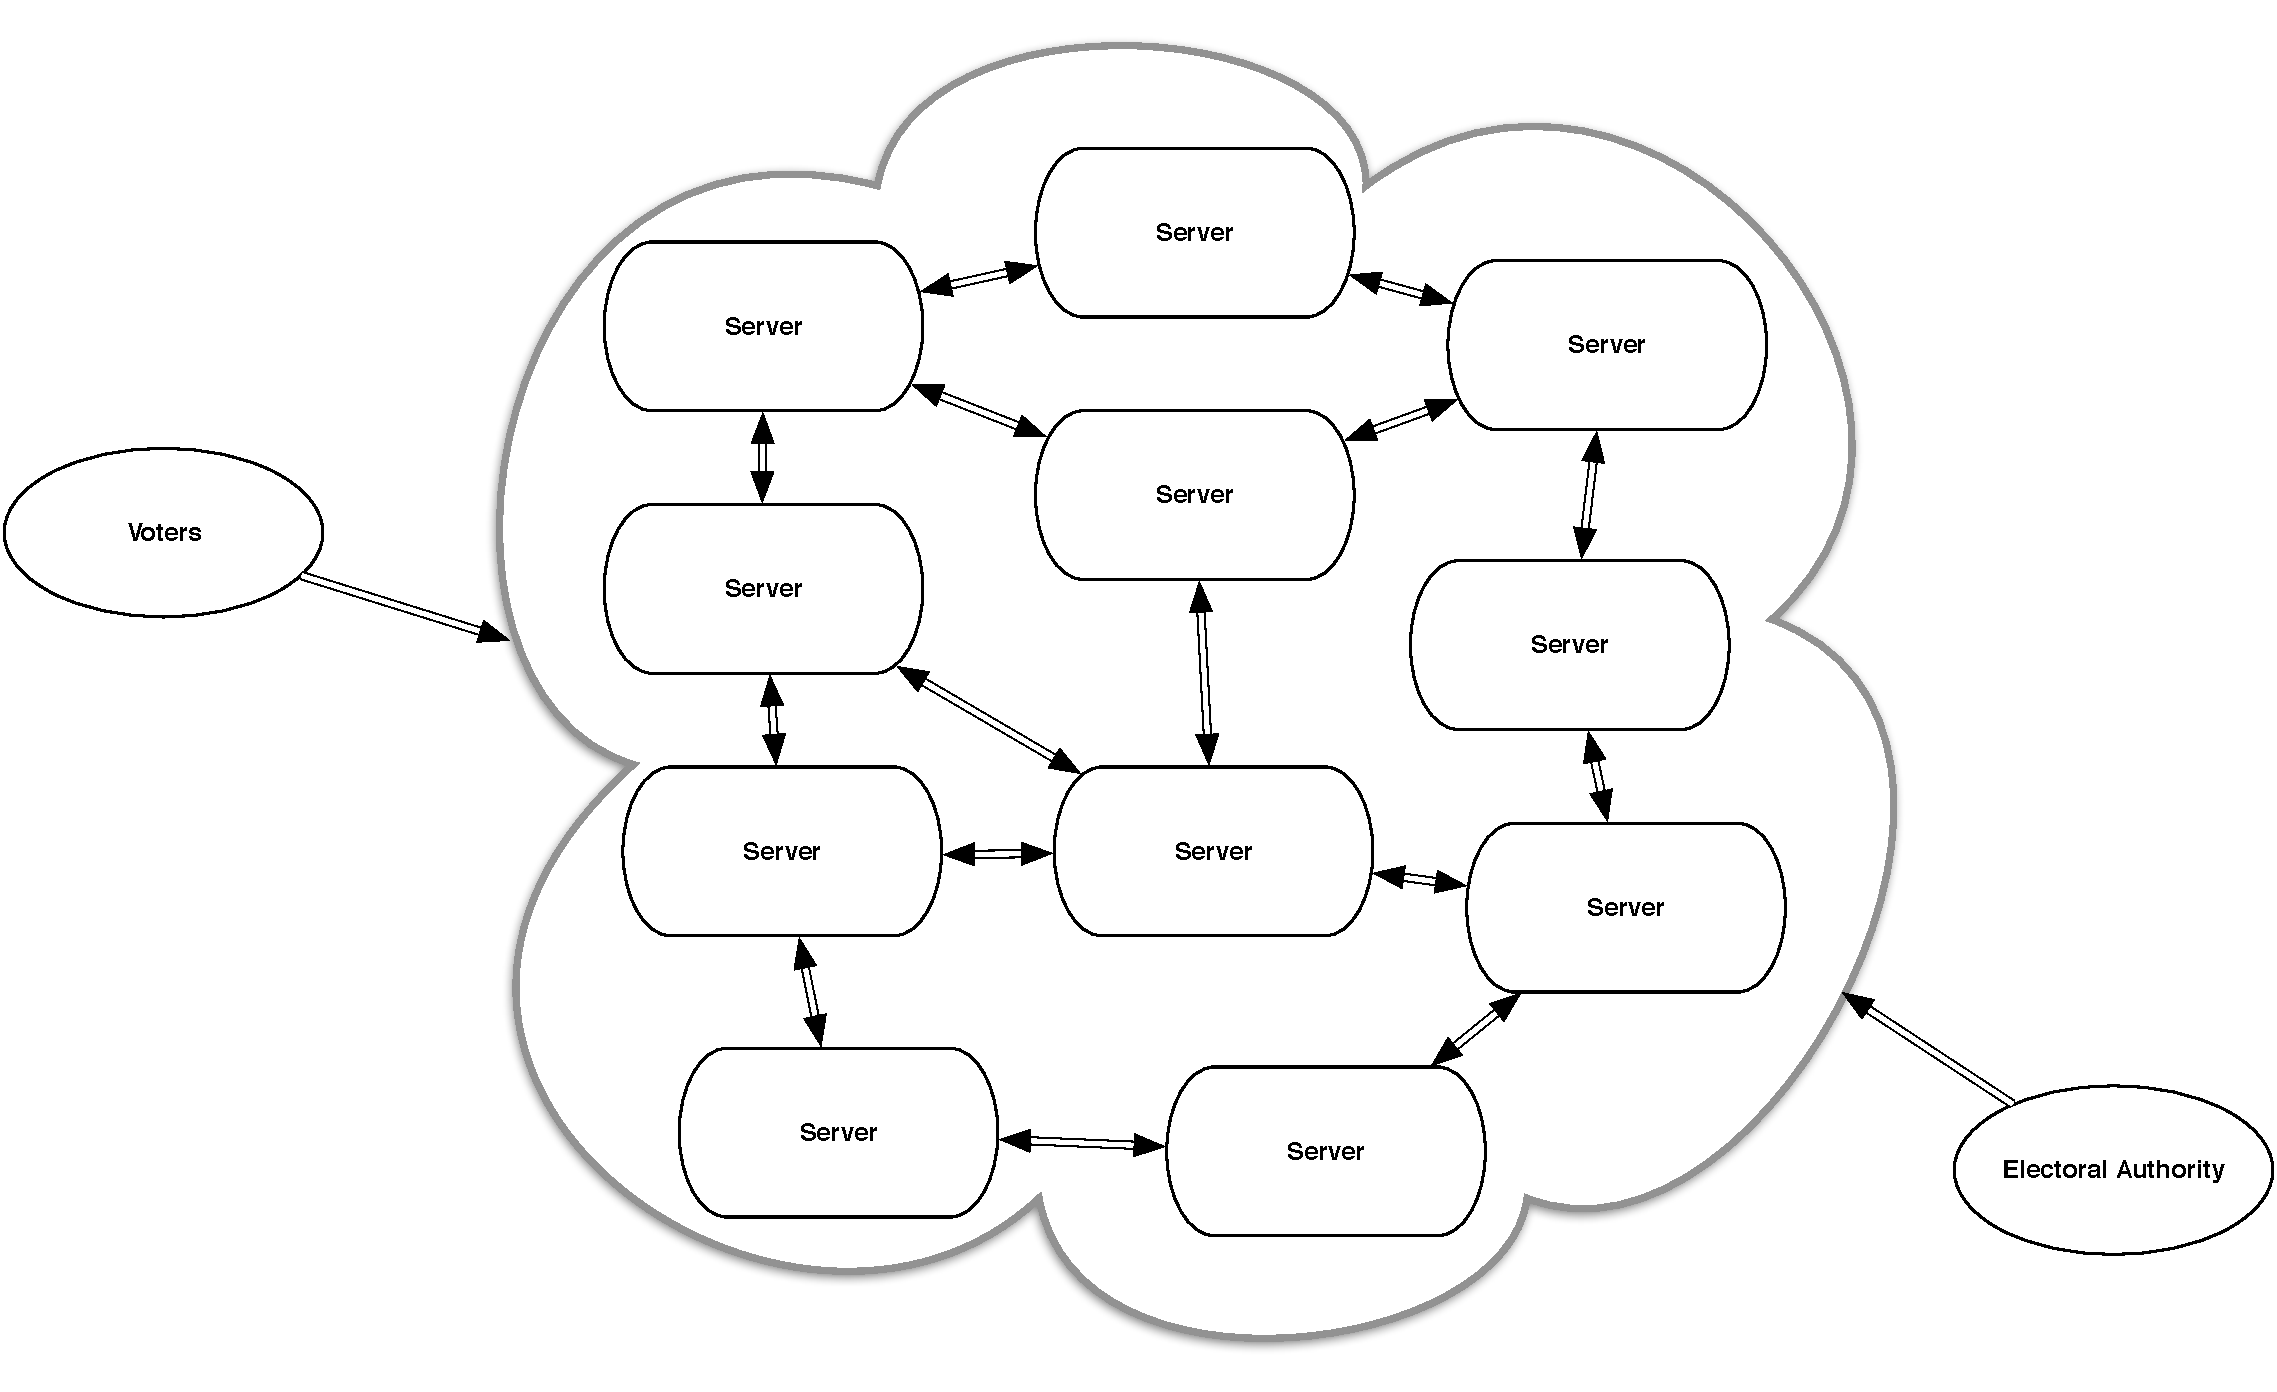
\includegraphics[width=6.5in]{architecture_resources/dynamic-cloud-large.pdf}
\end{center}
\caption{A dynamic cloud architecture with a larger number of servers.}
\label{figure:arch-dynamic-cloud-large}
\end{figure}

Effectively, a dynamic cloud deployment behaves similarly to a
deployment with a large fixed number of servers; the main difference
is that the number of servers is variable. This allows for the system
to initially consume minimal resources, expanding or contracting as
necessary (within the bounds of the dynamic cloud) to maintain
acceptable response time and availability in the face of elastic
demand.

Despite the use of the word ``cloud'', a dynamic cloud architecture
need not actually be deployed on a public cloud infrastructure;
private cloud infrastructures consisting of only trusted servers may
be built as necessary to support the system.\footnote{In the E2E-VIV
  context, however, public cloud infrastructures are likely preferable
  for economic reasons; it is virtually inconceivable that an
  electoral authority or its suppliers could build a cloud
  infrastructure with scale and reliability comparable to existing
  public cloud infrastructures at reasonable cost.}  Regardless of
whether the system is deployed on a trusted or public infrastructure,
authority in a dynamic cloud architecture follows either a fully
distributed or a hybrid model; some servers in the cloud may have
authority over others, or they may interact using consensus protocols
or similar mechanisms.

\begin{figure}[t!]
\begin{center}
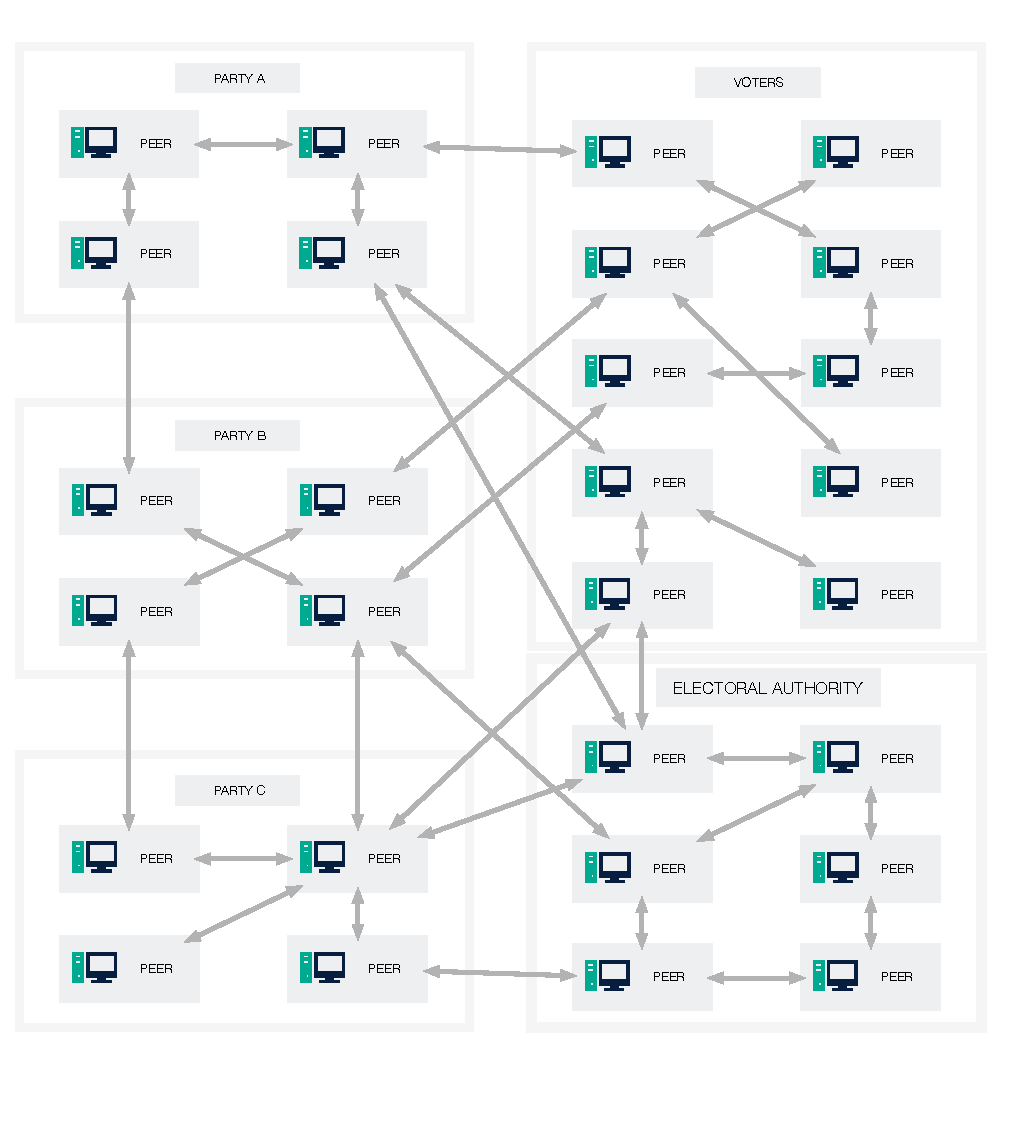
\includegraphics[width=6.5in]{architecture_resources/peer-to-peer.pdf}
\end{center}
\caption{A peer-to-peer architecture.}
\label{figure:arch-peer-to-peer}
\end{figure}

\subsection{Peer-to-Peer}

In all the architectural variants described so far, the system
presents itself as a single ``server'' regardless of its ``internal''
network topology. In a \emph{peer-to-peer} implementation, the
computational work of the system is distributed across all the
participants and there is no clearly defined distinction between
``client'' and ``server''. For example,
\autoref{figure:arch-peer-to-peer} depicts a peer-to-peer system with
a number of peers belonging to individual voters, some belonging to
political parties (A, B and C), and some belonging to the electoral
authority. The double-headed arrows in the figure represent
communication links among the peers; for example, if the upper-left
peer belonging to Party A needs to communicate with the lower-right
peer belonging to the electoral authority, it must send a message that
travels across at least 7 communication links. The communication links
in a peer-to-peer network typically change over time, based on each
peer's knowledge about its network environment and the locations of
other peers.

Authority in a peer-to-peer architecture is fully distributed. In the
case of an E2E-VIV system, the electoral authority would set up and
maintain some trusted peers as a way to ``bootstrap'' the peer-to-peer
network, and political organizations (parties, lobbying groups, etc.)
might also choose to maintain peers, perhaps with their own
implementations of the election software in a system designed with
open protocols and specifications, as a way of participating in the
electoral process and strengthening trust in the results. Individual
voters running the software on their own machines would also be peers
for the duration of their voting sessions (or longer, if they chose to
contribute to the management of the election by leaving the software
running); effectively, a peer-to-peer architecture is a way of
``crowdsourcing'' the resources required to run election system. 

A peer-to-peer architecture raises significant security concerns that
differ from those of the other architectures we have described. While
some of the computer systems controlled by the electoral authority
might be trusted, the vast majority of systems belonging to individual
voters or political organzations will certainly not be; it is
impossible to run a peer-to-peer E2E-VIV system using only trusted
computing resources.\footnote{This is true of ``pure'' peer-to-peer
  architectures of the type we are discussing in this section; an
  architecture where only the \emph{servers} interact in a
  peer-to-peer fashion while presenting a single interface or set of
  interfaces to clients can, as previously noted, be implemented on a
  fixed set of servers or in a dynamic cloud.} It is therefore
important to ensure that no corrupt peer, or set of corrupt peers, can
undetectably compromise election results, violate voter privacy, or
otherwise violate the E2E-VIV system requirements.

One way to address this problem is to employ a \emph{blockchain}, like
that used in Bitcoin and other cryptocurrencies, to log critical
election information (cast and spoiled ballots, the fact that a given
voter has voted in the election, etc.). A blockchain is a public
write-only ledger, collectively maintained by the peers in the system,
that records a sequence of events. The mechanism by which this
recording is done ensures that the peers reach a consensus about the
events that have occurred and their ordering, and that once an event
(such as the casting of an encrypted ballot) has been placed in the
ledger it can be neither modified nor reordered with respect to other
events. As long as more than half of the peer computing power in the
network is ``honest'' and follows the correct protocol, the integrity
of the ledger is guaranteed. At any given time, it is likely that the
computing power contributed by the electoral authority and
high-profile political organizations---which can be hosted on trusted,
closely-monitored computing systems---will vastly outweigh the
computing power contributed by individual voters during their ballot
casting sessions; moreover, the situation where more than half the
peer computing power is dishonest can be detected (by the honest part
of the network, or by external observers) and dealt with in various
ways. Thus, maintaining the integrity of a blockchain should be
reasonably straightforward in an E2E-VIV system. However, other aspects
of implementing a peer-to-peer architecture---such as distribution of
the computing client to voters and organizations, achieving sufficient
ease of use and performance, etc.---may prove more difficult.

\section{Summary}

As can be seen from the many architectural dimensions we have
described and the primary architectural variants we have briefly
discussed, there are many different ways in which an E2E-VIV system
could be designed and implemented. It is not clear which of the
primary variants would be the ``best'' option, nor is it clear exactly
what criteria would be used to make that determination among multiple
architectures that fulfill all the E2E-VIV requirements. Further
research and experimentation is therefore necessary to determine a
suitable path forward for E2E-VIV implementation and deployment.

